\section{Kuch. Nyutonning birinchi qonuni}

\begin{enumerate}

\item Jismning bir nuqtasiga 6 N va 8 N kuch bir-biriga nisbatan $180^\circ$
burchak ostida qo‘yilgan. Jismga ta’sir qiluvchi natijaviy kuchni toping (N).

\begin{enumerate}[label=\Alph*)]
\item 8
\item 6
\item 2
\item 10
\end{enumerate}


\item Arqon tortish musobaqasida to‘rt kishi ishtirok etmoqda.
Ulardan ikkitasi arqonni 250 N va 200 N kuch bilan o‘ng tomonga,
qolgan ikkitasi 350 N va 50 N kuch bilan chap tomonga tortmoqda. Teng ta’sir etuvchi kuch qanday? Arqon qaysi tomonga harakatlanadi?

\begin{enumerate}[label=\Alph*)]
\item 50 N, o‘ngga
\item 450 N, o‘ngga
\item 350 N, chapga
\item 850 N, o‘ngga
\end{enumerate}


\item Rasmda ko‘rsatilganidek $O$ nuqtaga ikkita $F_1$ va $F_2$
kuchlar ta’sir etmoqda. Ularning natijaviy kuchi qanday yo‘nalgan?

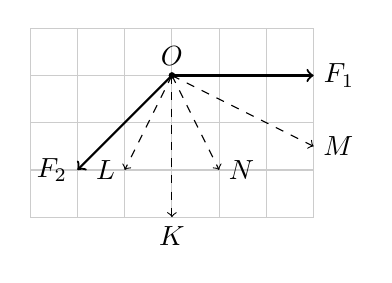
\begin{tikzpicture}[scale=0.6]

\draw[step=1cm,gray!40] (-3,-3) grid (3,1);

\fill (0,0) circle (2pt);
\node[above] at (0,0) {$O$};

\draw[->,thick] (0,0) -- (3,0) node[right] {$F_1$};
\draw[->,thick] (0,0) -- (-2,-2) node[left] {$F_2$};

\draw[dashed,->] (0,0) -- (-1,-2) node[left] {$L$};
\draw[dashed,->] (0,0) -- (1,-2) node[right] {$N$};
\draw[dashed,->] (0,0) -- (0,-3) node[below] {$K$};
\draw[dashed,->] (0,0) -- (3,-1.5) node[right] {$M$};

\end{tikzpicture}

\begin{enumerate}[label=\Alph*)]
\item N
\item L
\item M
\item K
\end{enumerate}


\item Rasmdagi $O$ nuqtaga qo‘yilgan kuchlarning teng ta’sir etuvchisi qanday (N)?

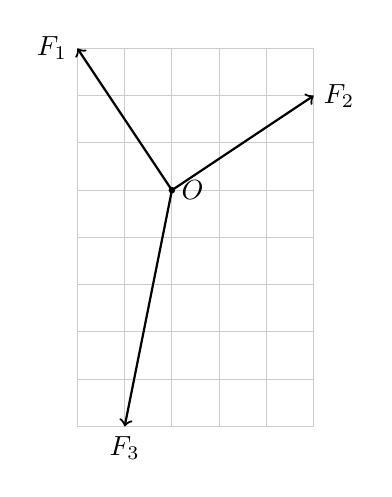
\begin{tikzpicture}[scale=0.6]

\draw[step=1cm,gray!40] (-2,-5) grid (3,3);

\fill (0,0) circle (2pt);
\node[right] at (0,0) {$O$};

\draw[->,thick] (0,0) -- (-2,3) node[left] {$F_1$};
\draw[->,thick] (0,0) -- (3,2) node[right] {$F_2$};
\draw[->,thick] (0,0) -- (-1,-5) node[below] {$F_3$};

\end{tikzpicture}

\begin{enumerate}[label=\Alph*)]
\item $2\sqrt{26}$
\item $2\sqrt{13}$
\item 0
\item $\sqrt{13}$
\end{enumerate}


\item Ushbu uchta kuchning teng ta’sir etuvchisini toping.

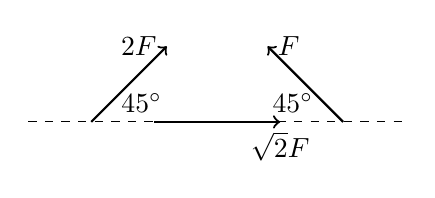
\begin{tikzpicture}[scale=0.8]

\draw[dashed] (-3,0) -- (3,0);

\draw[->,thick] (-2,0) -- (-0.8,1.2) node[left] {$2F$};
\draw[->,thick] (2,0) -- (0.8,1.2) node[right] {$F$};

\draw[->,thick] (-1,0) -- (1,0) node[below] {$\sqrt{2}F$};

\node at (-1.2,0.3) {$45^\circ$};
\node at (1.2,0.3) {$45^\circ$};

\end{tikzpicture}

\begin{enumerate}[label=\Alph*)]
\item $F$
\item $2F$
\item $\sqrt{2}F$
\item $3F$
\end{enumerate}


\item Ushbu uchta kuchning teng ta’sir etuvchisini toping.

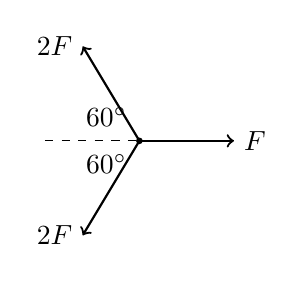
\begin{tikzpicture}[scale=0.6]

\draw[dashed] (-2,0) -- (2,0);

\fill (0,0) circle (2pt);

\draw[->,thick] (0,0) -- (2,0) node[right] {$F$};
\draw[->,thick] (0,0) -- (-1.2,2) node[left] {$2F$};
\draw[->,thick] (0,0) -- (-1.2,-2) node[left] {$2F$};

\node at (-0.7,0.5) {$60^\circ$};
\node at (-0.7,-0.5) {$60^\circ$};

\end{tikzpicture}

\begin{enumerate}[label=\Alph*)]
\item $F$
\item $\sqrt{3}F$
\item $\sqrt{2}F$
\item $2\sqrt{3}F$
\end{enumerate}


\item $M$ moddiy nuqtaga $F_1, F_2, F_3$ va $F_4$ kuchlar rasmda ko‘rsatilgandek ta’sir qilmoqda.
Moddiy nuqta qaysi tomonga va qanday kuch ta’siri ostida harakatlanadi?

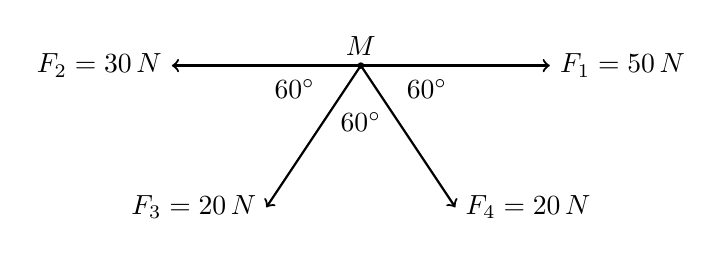
\begin{tikzpicture}[scale=0.6]

\fill (0,0) circle (2pt);
\node[above] at (0,0) {$M$};

\draw[->,thick] (0,0) -- (4,0) node[right] {$F_1=50\,\text{N}$};
\draw[->,thick] (0,0) -- (-4,0) node[left] {$F_2=30\,\text{N}$};

\draw[->,thick] (0,0) -- (-2,-3) node[left] {$F_3=20\,\text{N}$};
\draw[->,thick] (0,0) -- (2,-3) node[right] {$F_4=20\,\text{N}$};

\node at (-1.4,-0.5) {$60^\circ$};
\node at (1.4,-0.5) {$60^\circ$};
\node at (0,-1.2) {$60^\circ$};

\end{tikzpicture}

\begin{enumerate}[label=\Alph*)]
\item $F_2$ yo‘nalishda 10 N
\item $F_1$ yo‘nalishda 20 N
\item $F_3$ yo‘nalishda 30 N
\item $F_4$ yo‘nalishda 40 N
\end{enumerate}


\item Ushbu to‘rtta kuchning teng ta’sir etuvchisini toping (N).

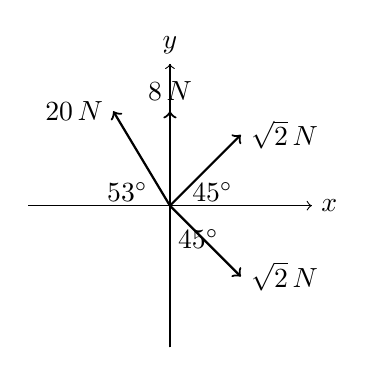
\begin{tikzpicture}[scale=0.6]

\draw[->] (-3,0) -- (3,0) node[right] {$x$};
\draw[->] (0,-3) -- (0,3) node[above] {$y$};

\draw[dashed] (-3,0) -- (3,0);
\draw[dashed] (0,-3) -- (0,3);

\draw[->,thick] (0,0) -- (0,2) node[above] {$8\,\text{N}$};

\draw[->,thick] (0,0) -- (1.5,1.5) node[right] {$\sqrt2\,\text{N}$};
\draw[->,thick] (0,0) -- (1.5,-1.5) node[right] {$\sqrt2\,\text{N}$};

\draw[->,thick] (0,0) -- (-1.2,2) node[left] {$20\,\text{N}$};

\node at (-0.9,0.3) {$53^\circ$};
\node at (0.9,0.3) {$45^\circ$};
\node at (0.6,-0.7) {$45^\circ$};

\end{tikzpicture}

\begin{enumerate}[label=\Alph*)]
\item 34
\item 89
\item 26
\item 18
\end{enumerate}


\item Quyidagi $O$ nuqtaga qo‘yilgan kuchlarning teng ta’sir etuvchisini toping (N).

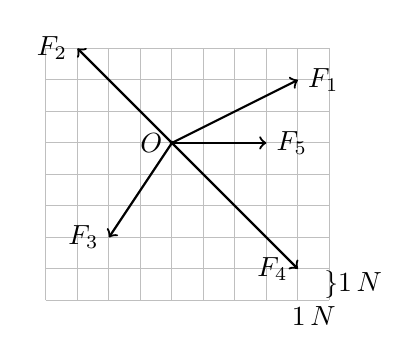
\begin{tikzpicture}[scale=0.4]

\draw[step=1cm,gray!50] (-4,-5) grid (5,3);

\fill (0,0) circle (2pt);
\node[left] at (0,0) {$O$};

\draw[->,thick] (0,0) -- (4,2) node[right] {$F_1$};
\draw[->,thick] (0,0) -- (-3,3) node[left] {$F_2$};
\draw[->,thick] (0,0) -- (-2,-3) node[left] {$F_3$};
\draw[->,thick] (0,0) -- (4,-4) node[left] {$F_4$};
\draw[->,thick] (0,0) -- (3,0) node[right] {$F_5$};

\node at (5.75,-4.5) {$\}1\,\text{N}$};
\node at (4.5,-5.5) {$1\,\text{N}$};

\end{tikzpicture}

\begin{enumerate}[label=\Alph*)]
\item $\sqrt{22}$
\item $2\sqrt{10}$
\item 15
\item 40
\end{enumerate}


\item Moddiy nuqtaga ta’sir etuvchi kuchlar muvozanatda bo‘lgandagi harakatlar qaysi grafiklarda tasvirlangan?

\begin{tikzpicture}[scale=0.9]

% 1-grafik
\begin{scope}
\draw[->] (0,0) -- (2.5,0) node[right] {$t$};
\draw[->] (0,0) -- (0,2.5) node[above] {$S$};
\draw[thick,smooth] plot coordinates {(0,0)(0.8,0.2)(1.5,0.8)(2,2)};
\node at (-0.3,2) {1)};
\end{scope}

% 2-grafik
\begin{scope}[xshift=3.5cm]
\draw[->] (0,0) -- (2.5,0) node[right] {$t$};
\draw[->] (0,0) -- (0,2.5) node[above] {$v$};
\draw[thick] (0,0) -- (2,2);
\node at (-0.3,2) {2)};
\end{scope}

% 3-grafik
\begin{scope}[xshift=7cm]
\draw[->] (0,0) -- (2.5,0) node[right] {$t$};
\draw[->] (0,0) -- (0,2.5) node[above] {$x$};
\draw[thick] (0,1.2) -- (2.2,1.2);
\node at (-0.3,2) {3)};
\end{scope}

% 4-grafik
\begin{scope}[xshift=10.5cm]
\draw[->] (0,0) -- (2.5,0) node[right] {$t$};
\draw[->] (0,0) -- (0,2.5) node[above] {$x$};
\draw[thick] (0,1) -- (2.2,2);
\node at (-0.3,2) {4)};
\end{scope}

\end{tikzpicture}

\begin{enumerate}[label=\Alph*)]
\item 1,2
\item 3,4
\item 2,4
\item 2,3,4
\end{enumerate}


\item Nyutonning birinchi qonunini tavsiflovchi ifodani ko‘rsating.

\begin{enumerate}[label=\Alph*)]
\item $v=\text{const},\; F=0$
\item $v=\text{const},\; v=at$
\item $F=\text{const},\; v=v_0+at$
\item $F=0,\; s=\text{const}$
\end{enumerate}

\item Avtomobil to‘g‘ri gorizontal yo‘lda o‘zgarmas tezlik bilan harakatlanmoqda. 
Unga ta’sir qilayotgan kuchlarning teng ta’sir etuvchisi haqida nima deyish mumkin?

\begin{enumerate}[label=\Alph*)]

\item og‘irlik va ishqalanish kuchlari yig‘indisiga teng
\item og‘irlik kuchiga teng va yuqoriga yo‘nalgan
\item qarshilik kuchiga teng va harakat yo‘nalishiga qarshi yo‘nalgan
\item TJY
\end{enumerate}


\end{enumerate}

\begin{table}[ht]
\centering
\begin{tabular}{|c|c|c|c|c|c|c|c|c|c|}
\hline
1c & 2a & 3a & 4c & 5d & 6a & 7d & 8c & 9b & 10d \\ \hline
11a & 12d &  &  &  &  &  &  &  &  \\ \hline
\end{tabular}
\end{table}










